\minitoc

\vfill

In this chapter, the first building bricks of our approach are presented: the error definitions.
We proceed by reprising the main consequences of the constraints that were imposed for our evaluation approach in subsection ~\ref{subsec::introduction::contributions::positioning}.
These will determine the desired properties that are seeked in this work.\\

We establish, in Section~\ref{sec::semantic_evaluation::general_framework} a general structure of the error taxonomy.
Section~\ref{sec::semantic_evaluation::overhead} details an implementation of this general stucture for the overhead automatic modeling case.
After discussing some properties of the chosen error defnitions, we explain, in the final Section~\ref{sec::semantic_evaluation::label_extraction}, how the final labels are extracted from the error taxonomy based on the quality evaluation requirements.

\clearpage

\section{The general framework}
    \label{sec::semantic_evaluation::general_framework}
    As stated previously in Section~\ref{subsec::introduction::contributions::positioning}, a semantic evaluation implies a categorization of errors affecting building models.
    In the same subsection, we discussed the desired properties in order to achieve a \textbf{large-scale} and \textbf{automatic} semantic evaluation.
    Before delving into details, we first examine the implications of such properties on error definitions in Section~\ref{subsec::semantic_evaluation::general_framework::hierarchization_moderularity}.
    Next, Section~\ref{subsec::semantic_evaluation::general_framework::error_classification} presents a general layout of the proposed error taxonomy.

    \subsection{Hierarchization and modularity}
        \label{subsec::semantic_evaluation::general_framework::hierarchization_moderularity}
        The goal of this subsection is to state the desired characteristics in the categorization of building model defects based on the discussion in Section~\ref{subsec::introduction::contributions::positioning}.
        We introduce first two notions: generalizability and exhaustivity.
        These are directly linked to the \textbf{large-scale} aspect of the evaluation approach.
        These are implemented in the error categorization based on two principles: hierarchization and modularity.

        \subsubsection{The generalizability \textit{vs.} exhaustivity compromise.}
            In Section~\ref{subsec::introduction::contributions::positioning}, we have seen how the \textbf{large-scale} constraint on the quality evaluation approach entails the method's robustness to changes in the urban scene as well as to the pipeline behind the evaluated model.
            The first condition implies the proposed error categorization capacity to be generalizable: the ability to describe defects of building models unhindered by the specificities of one scene or another.
            The second conveys the exhaustivity of the evaluation: the power to take into account all possible errors that a building model can be affected by, free of any consideration of its origin.\\

            The two notions are condradictory.
            At one hand, every possible defect should be accounted for at all levels.
            This may be possible through a meticulous analysis of models from a specific area.
            In fact, similar to the procedural modeling approaches, building model errors could be portayed relying on expert knowledge.
            For instance, Haussmann style building modeling defects could be described exhaustively.
            Eventhough these errors would be sufficient for a small disctrict in downtown Paris, they are clearly not comprehensive enough to encorporate cases from other types of buildings like in La D\'efense, just \SI{3}{\km} away of Paris, let alone ones from Timbuktu, Mali.\\

            On the other, the categorization has to stay always relevant no matter the origin of those models.
            This can be, for example, achieved based on a list of errors that are common across all possible building types.
            However, this has the disadvantage of not covering all the instances specific one input method or another.
            A compromise has to be reached in the definition of errors between generalizability and exhaustivity.
        
        \subsubsection{General structure.}
            We introduce a hierarchical structure to categorize errors in order to mitigate the last point.
            The higher in the ladder the error is, the more generalizability (and less exhaustivity) is achieved.
            At the same hierarchical level, to avoid having to exhaustively list all possible errors, the identified defects are described modularly based on some predefined independent errors.
            This helps cover a wide range of possible defects while the basic errors are chosen to be as generalizable as possible.
            Hierarchization and modularity are the main ingredients in our proposed flexible framework.\\

            To implement these properties for the error taxonomy, we rely on two criteria for error compilation: the input building model \gls{acr::lod} and the error semantic precision level, named henceforth \texttt{finesse} (cf. Figure~\ref{fig::taxonomy}).
            Different degrees of \texttt{finesse} describe, from coarse to fine, the specificity of defects.
            \texttt{Finesse} degrees corresponds to error hierarchy levels.
            The \gls{acr::lod} is used, on the other hand, to differenciate between errors in the same specificity (or \texttt{finesse}) level.
            Multiple errors at the same \texttt{finesse} can indeed affect the same building.
            For instance, topological defects almost always induce (and hence co-occur) with geometrical ones.\\
            Errors with maximal \texttt{finesse} are called \texttt{atomic} errors.
            \texttt{Atomic} errors are to be intuitively correlated to independent actions needed by an operator or an algorithm so as to correct the model.

    \subsection{A general classification of errors}
        \label{subsec::semantic_evaluation::general_framework::error_classification}
        Herein, based on the previous discussion, a general layout is detailed for building model evaluation.

        At a first level, model qualifiability is studied.
        In fact, aside from formatting issues or geometric inconsistencies~\parencite{ledoux2018val3dity}, other reasons make building models unqualifiable.
        For instance, buildings can be occluded by vegetation and thus cannot be assessed from most of the remote sensing data sources.
        Generally speaking, input models can be impaired by some pathological cases that are outside our evaluation framework.
        In consequence, \texttt{Qualifiable} models are distinguished here from \texttt{Unqualifiable} buildings.
        This first level corresponds to a \texttt{finesse} equal to 0.\\
        At the \texttt{finesse} level 1, we predict the correctness of all qualifiable buildings.
        It is the lowest semantization level at which the evaluation of a model is expressed.
        Then, a model is either \texttt{Valid} or \texttt{Erroneous}.
        Most state-of-the-art evaluation methods address errors up to this level.\\
        Model errors are grouped into two families depending on the underlying \gls{acr::lod}.
        The first family of errors \texttt{Building Errors} affects the building in its entirety.
        It corresponds to an accuracy evaluation at \gls{acr::lod}-0 (footprint errors) $\cup$ \gls{acr::lod}-1 (height/geometric error).\\
        At the next \gls{acr::lod}-2, the family \texttt{Facet Errors} gathers defects that can alter the facet accuracy of fa\c{c}ades or roofs (\gls{acr::lod}-2) as well as superstructures and openings (\gls{acr::lod}-3).\\
        Each family contains \texttt{atomic} errors of maximal \texttt{finesse} equal to 3.
        Although they can co-occur in the same building model and across different families, these errors are semantically independent\footnote{As mentioned before, they relate, instinctively, to independent corrective tasks.}.
        They represent specific topological or geometric defects.
        Topological errors translate inaccurate structural modeling, while geometric defects raise positioning infidelity.\\

        The general structure is not fixed and can evolve to adapt to more cases.
        In fact, instead of grouping \gls{acr::lod}-2 and \gls{acr::lod}-3 errors, the latter can be made into a different family that can be called \texttt{Superstructure Errors}.
        Due to the lack of sufficient observations, we did not make this choice in order to guaranty the generalizability of the taxonomy.
        Another alternative consists, for instance, in gathering error families by resolution: this will produce a continuum of errors families going from the coarsest level that would correspond to \texttt{Building Errors} to the finest possible one.
        This last option, although offering an exhaustive and potentially generalizable taxonomy, was ruled out since it does not provide a truly semantic description of the errors.
        Regarding \texttt{finesse}, it is also possible to have additional levels.
        The maximal level of 3 was chosen in order to preserve the generalizability of the taxonomy, since the more specific the error categorization is, the more observations are needed to define the corresponding errors.

        \begin{figure}[htbp]
            \begin{center}
                \includestandalone[mode=buildnew, width=\textwidth]{figures/taxonomy_tree}
                \caption{
                    \label{fig::taxonomy} 
                    The proposed taxonomy structure.
                    In our case of very high resolution overhead image modeling, only two family errors are depicted.
                    At \texttt{finesse} level 2, hierarchization is possible: an \textbf{exclusivity} parameter can thus act.
                    However, it is not the case at the \texttt{atomic} errors level since they are independent.
                }
            \end{center}
        \end{figure}

\section{Application to the overhead case}
    \label{sec::semantic_evaluation::overhead}
    Our observations were based on large datasets of \gls{acr::3d} models of buildings reconstructed automatically out of \gls{acr::vhr} images or, if available, \gls{acr::lidar} point clouds.
    The framework introduced in the previous subsection was applied to our special case.
    To do so, let us define the \texttt{atomic} errors before discussing their properties.

    \subsection{Atomic error definitions}
        \label{subsec::semantic_evaluation::overhead::atomic}
        In the template structure presented in Section~\ref{subsec::semantic_evaluation::general_framework::error_classification}, were left out the \texttt{atomic} error definitions.
        Indeed, since they represent the most specific level, their choice is critical to guaranty both the desired exhaustivity and generalizability.
        We conducted a thorough inspection of all defects that we detected in our datasets and came up with the following definitions (cf. Figures~\ref{fig::taxonomy}).
        Eventhough these errors were defined based on models of buildings computed out of overhead acquired data at large scales, we think they are exhaustive enough to describe the quality of models in other settings (fa\c{c}ade modeling, manually plotted \gls{acr::3d} models).

        \subsubsection{\texttt{Building Errors} family.}
            Herein are presented the \texttt{atomic} errors regarding the \gls{acr::lod}-0 and \gls{acr::lod}-1 aspects.

            \paragraph{\texttt{\acrlong*{acr::bus}}.}
                \texttt{\gls{acr::bus}} corresponds to the case where two or more buildings are modeled as one.
                In Figure~\ref{fig::bus}, two distinct buildings were identified as one building, eventhough they can be visually distinguished.\\

                \begin{figure}[htbp]
                    \centering
                    \ffigbox[\textwidth]{
                        \begin{subfloatrow}
                            \ffigbox[.5\textwidth]{
                                \includestandalone[mode=buildnew, width=.45\textwidth]{figures/errors/building/bos}
                            }{
                                \caption{
                                    \label{subfig::gt_bus_3d}
                                    Ground truth \gls{acr::3d} models.
                                    The different buildings are in different colors: blue and green.
                                }
                            }
                            \ffigbox[.5\textwidth]{
                                \includestandalone[mode=buildnew, width=.45\textwidth]{figures/errors/building/bus}
                            }{
                                \caption{
                                    \label{subfig::bus_3d}
                                    \gls{acr::3d} models of the buildings fused into one model.
                                }
                            }
                        \end{subfloatrow}
                        \vskip1em
                        \begin{subfloatrow}
                                \centering
                                \ffigbox[.75\textwidth]{
                                    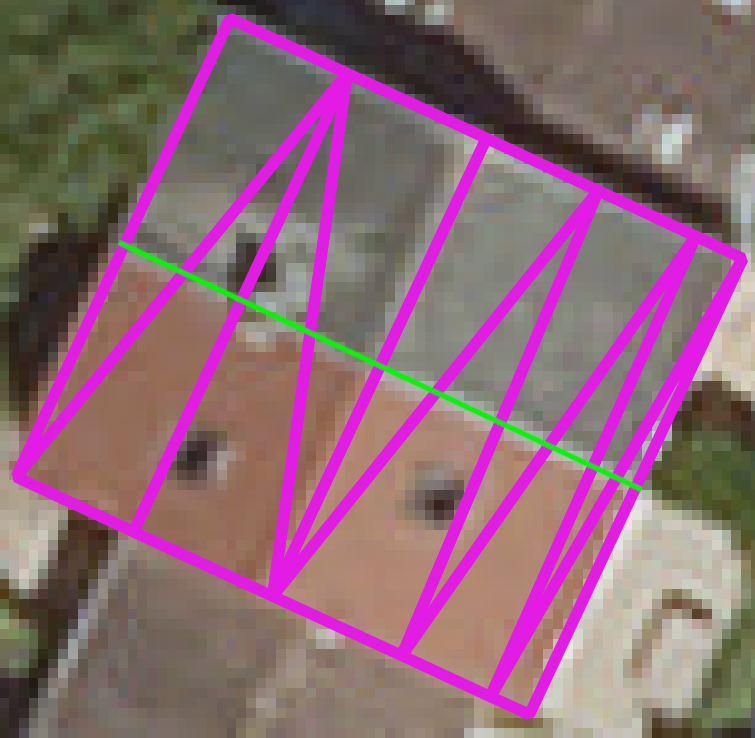
\includegraphics[width=.5\textwidth]{images/errors/building/under_segmentation}
                                }{
                                    \caption{
                                        \label{subfig::bus_2d}
                                        Nadir projection of an erroneous building superposed on the corresponding orthoimage.
                                        We can recognize, based on the color differences of roof tiles, the existance of two buildings instead of one.
                                    }
                                }
                        \end{subfloatrow}
                    }{
                        \caption{
                            \label{fig::bus}
                            Illustration of a \gls{acr::bus} error.
                        }
                    }
                \end{figure}

                This is a very common error which results from a faulty footprint of the building.
                The latter is either retrieved automatically during the modeling~\parencite{lafarge2012creating}, or is provided as input~\parencite{durupt2006automatic}.
                The first case is the most error inducing one as it relies on extrinsic large-scale remote sensing data that are devoid of semantics.
                The second one is expected to be more close to the reality, but can be unsuitable if the footprints are outdated or too generalized, as discussed in Section~\ref{subsec::state_of_the_art::building_modeling::building_extraction}.

            \paragraph{\texttt{\acrlong*{acr::bos}}.}
                \texttt{\gls{acr::bos}} corresponds to the case where one building is subdivided into two or more.
                This is the opposite of the previous situation.
                Figure~\ref{fig::bos_2d} shows a single building that, when modeled, was subdivided into three parts.\\

                \begin{figure}[htbp]
                    \centering
                    \ffigbox[\textwidth]{
                        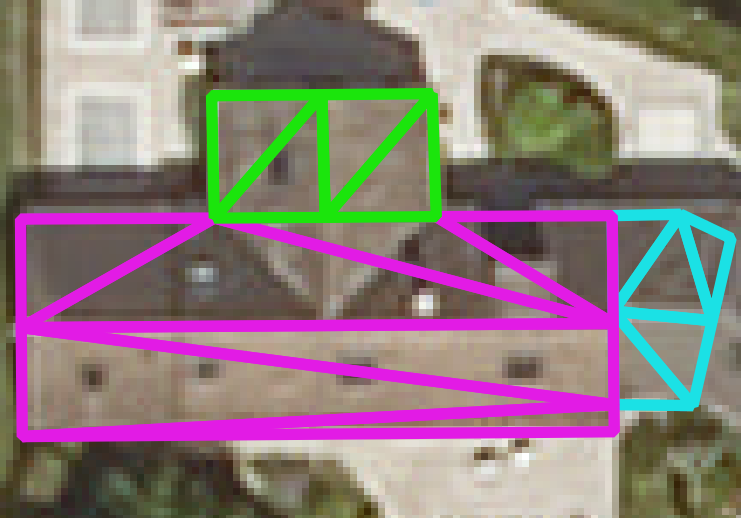
\includegraphics[width=.5\textwidth]{images/errors/building/over_segmentation}
                    }{
                        \caption{
                            \label{fig::bos_2d}
                            This a nadir projection of a single building that was modeled into three different ones depicted here in three different colors.
                        }
                    }
                \end{figure}

                This is also a very common error.
                It is the consequence of the same reasons as the under segmentation that was discussed earlier.
                Both these errors are highly semantic and ,thus, creates confusion between both classes.
                Depending on the chosen semantics, a building part (in the sense of CityGML) can be also considered as a single building in other cases.
                These defects depend, actually, on the human perception of buildings and are more ambiguous by nature, unless \textit{explicit} semantic information is provided along the geometry fo the model.
                In fact, there is no combination of geometric characteristic that can help separate buildings, such as convexity or compactness.
                This issue is expected to weight negatively on the predictive capacity of the proposed evaluation approach as will be further studied in Section~\ref{sec::experiments::scalability}.

            \paragraph{\texttt{\acrlong*{acr::bib}}.}
                \texttt{\gls{acr::bib}} corresponds to the case where at least one building footprint border is incorrectly located.
                A sample is shown in Figure~\ref{fig::bib}.\\

                \begin{figure}[htbp]
                    \centering
                    \ffigbox[\textwidth]{
                        \begin{subfloatrow}
                            \ffigbox[.5\textwidth]{
                                \includestandalone[mode=buildnew, width=.45\textwidth]{figures/errors/building/correct_bib}
                            }{
                                \caption{
                                    \label{subfig::gt_bib_3d}
                                    Ground truth \gls{acr::3d} model.
                                }
                            }
                            \ffigbox[.5\textwidth]{
                                \includestandalone[mode=buildnew, width=.45\textwidth]{figures/errors/building/bib}
                            }{
                                \caption{
                                    \label{subfig::bib_3d}
                                    \gls{acr::3d} models with an imprecise border (in red).
                                }
                            }
                        \end{subfloatrow}
                        \vskip1em
                        \begin{subfloatrow}
                                \centering
                                \ffigbox[.75\textwidth]{
                                    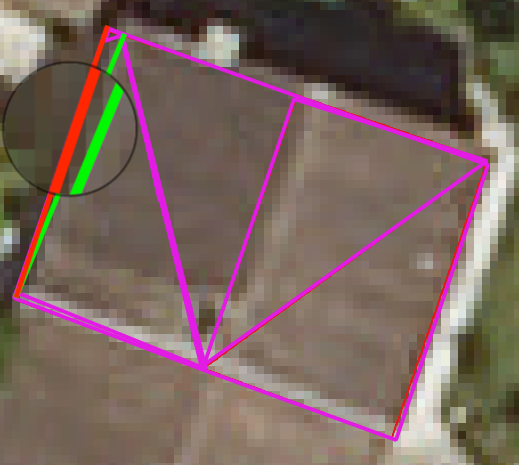
\includegraphics[width=.5\textwidth]{images/errors/building/border}
                                }{
                                    \caption{
                                        \label{subfig::bib_2d}
                                        In red is the reconstructed model border that is misestimated, as can be checked in the orthoimage.
                                        We can distinguish in green the actual edge using a Nadir projection.
                                    }
                                }
                        \end{subfloatrow}
                    }{
                        \caption{
                            \label{fig::bib}
                            Illustration of a \texttt{\gls{acr::bib}} error.
                        }
                    }
                \end{figure}

                This is a purely geometric error that is caused by an imprecise footprint.
                Actually, semantics play a role as \texttt{\gls{acr::bib}} is mainly linked to the end user preferences: one can ignore errors up to a certain threshold. 
                As with previous \texttt{\gls{acr::bus}} and \texttt{\gls{acr::bos}} errors, the footprint border precision is understandably susceptible on the quality of the input data used for modeling.
                It is also expected that the error detection precision will hinge on the resolution of the used reference data and its registration accuracy.
                Regarding automatic modeling methods, border imprecision can be attributed to the quality of the used edge detection algorithms~\parencite{baillard1999automatic,werner2002new,nan2015template} or inaccurate surface estimation\footnote{
                    The border is computed as intersection of the detected surfaces.
                }~\parencite{durupt2006automatic,xiong2014graph}.
                Outside the scope this study, one can try also to estimate the imprecision so as to correct the reconstruction.

            \paragraph{\texttt{\acrlong*{acr::bit}}.}
                \texttt{\gls{acr::bit}} corresponds to the case where the building footprint suffers from topological defects.
                Modeled as a \gls{acr::2d} flat surface, the cases that fall into this label are:
                \begin{description}
                    \item[Missing inner court:] It corresponds to a missing hole (cf. Figure~\ref{subfig::building_hole});
                    \item[Inaccurate border shape:] It is due to a wrong primitive fitting: the shape of the footprint can be better described by a different geometrical shape.
                            Figure~\ref{subfig::bit_2d} gives an example where the polygon has a wrong number of sides.
                            Another case is where a circular footprint can be approximated by a polygon.
                \end{description}

                \begin{figure}[htbp]
                    \centering
                    \ffigbox[\textwidth]{
                        \begin{subfloatrow}
                            \ffigbox[.5\textwidth]{
                                \includestandalone[mode=buildnew, width=.45\textwidth]{figures/errors/building/correct_bit}
                            }{
                                \caption{
                                    \label{subfig::gt_bit_3d}
                                    Ground truth \gls{acr::3d} model.
                                }
                            }
                            \ffigbox[.5\textwidth]{
                                \includestandalone[mode=buildnew, width=.45\textwidth]{figures/errors/building/bit}
                            }{
                                \caption{
                                    \label{subfig::bit_3d}
                                    \gls{acr::3d} models with an inaccurate topology.
                                    The concerned borders are in yellow.
                                }
                            }
                        \end{subfloatrow}
                        \vskip1em
                        \begin{subfloatrow}
                                \centering
                                \ffigbox[.75\textwidth]{
                                    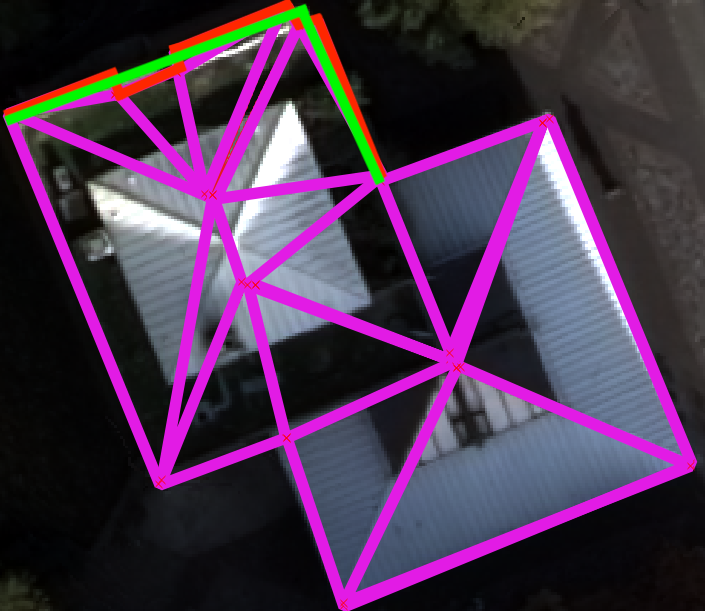
\includegraphics[width=.5\textwidth]{images/errors/building/topology}
                                }{
                                    \caption{
                                        \label{subfig::bit_2d}
                                        The nadir projection comparison with the corresponding orthoimage gives away (in green) the correct footprint shape compared to the one that was reconstructed (in red).
                                    }
                                }
                        \end{subfloatrow}
                    }{
                        \caption{
                            \label{fig::bit}
                            Illustration of a \texttt{\gls{acr::bit}} error.
                        }
                    }
                \end{figure}

                This error, as the earlier one, is a result of a defective edge estimation.
                The main difference between both of them states in the fact that \texttt{\gls{acr::bib}} is geometric in nature while \texttt{\gls{acr::bit}} is topological.
                Both errors are independent and can overlap.

            \paragraph{\texttt{\acrlong*{acr::big}}.}
                \texttt{\gls{acr::big}} corresponds to the case of inaccurate building geometric estimation.

                \begin{figure}[htbp]
                    \centering
                    \ffigbox[\textwidth]{
                        \begin{subfloatrow}
                            \ffigbox[.5\textwidth]{
                                \includestandalone[mode=buildnew, width=.45\textwidth]{figures/errors/building/correct_big}
                            }{
                                \caption{
                                    \label{subfig::gt_big_3d}
                                    Ground truth \gls{acr::3d} model.
                                }
                            }
                            \ffigbox[.5\textwidth]{
                                \includestandalone[mode=buildnew, width=.45\textwidth]{figures/errors/building/big}
                            }{
                                \caption{
                                    \label{subfig::big_3d}
                                    \gls{acr::3d} models with an imprecise height estimation.
                                }
                            }
                        \end{subfloatrow}
                    }{
                        \caption{
                            \label{fig::big}
                            Illustration of a \texttt{\gls{acr::big}} error.
                        }
                    }
                \end{figure}

                Up to \gls{acr::lod}-1, it coincides with height imprecision, as depicted in Figure~\ref{fig::big}.
                This is yet again a geometric error.
                Semantics play a role in the definition of the height of a building.
                It can be defined as the height at the highest point, the mediane height or any other valid alternative.
                In case of evaluating at higher than \gls{acr::lod}-2, this error is not reported as it becomes redundant with errors delineated below.
                In fact, if a geometric error is detected at the facet level then it will naturally impact negatively on the geometry of the model as a whole.
            
        \subsubsection{\texttt{Facet Errors} family.}
            In this Section, \gls{acr::lod}-2 and \gls{acr::lod}-3 corresponding \texttt{atomic} errors are presented.

            \paragraph{\texttt{\acrlong*{acr::fus}}.}
                \texttt{\gls{acr::fus}} corresponds to the case where one facet is subdivided into two or more facets.
                This is the same kind of error as \texttt{\gls{acr::bus}} but at the facet level.\\

                \begin{figure}[htbp]
                    \centering
                    \ffigbox[\textwidth]{
                        \begin{subfloatrow}
                            \ffigbox[.5\textwidth]{
                                \includestandalone[mode=buildnew, width=.45\textwidth]{figures/errors/facet/correct_fos_fus_fib_fig}
                            }{
                                \caption{
                                    \label{subfig::gt_fus_3d}
                                    Ground truth \gls{acr::3d} model.
                                }
                            }
                            \ffigbox[.5\textwidth]{
                                \includestandalone[mode=buildnew, width=.45\textwidth]{figures/errors/facet/fus}
                            }{
                                \caption{
                                    \label{subfig::fus_3d}
                                    \gls{acr::3d} model with a \texttt{\gls{acr::fus}} error.
                                    The erroneous facet is colored in blue.
                                }
                            }
                        \end{subfloatrow}
                        \vskip1em
                        \begin{subfloatrow}
                                \centering
                                \ffigbox[.75\textwidth]{
                                        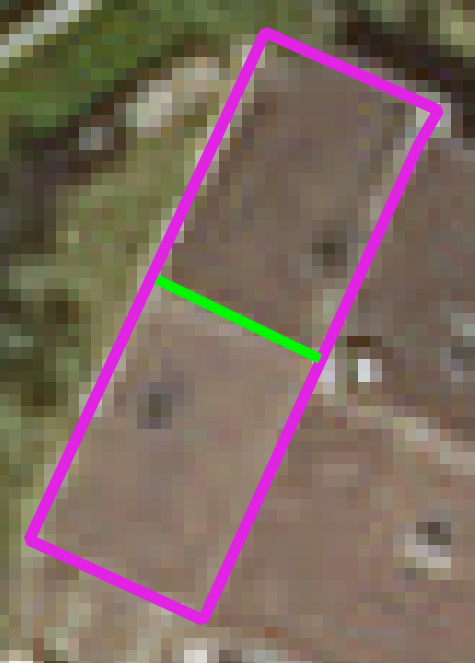
\includegraphics[width=.5\textwidth, width=.5\textwidth]{images/errors/facet/under_segmentation}
                                }{
                                    \caption{
                                        \label{subfig::fus_2d}
                                        Nadir projection of an erroneous building superposed on the corresponding orthoimage.
                                        It shows a case where a higher neighboring building part can drive a misestimation of both facet planes which end up confused in one flat roof.
                                        The line segment highlighted in green gives away the fact that the roof was undersegmented.
                                    }
                                }
                        \end{subfloatrow}
                    }{
                        \caption{
                            \label{fig::fus}
                            Illustration of a \texttt{\gls{acr::fus}} error.
                        }
                    }
                \end{figure}

                Usually automatic reconstruction methods rely on an initial surface (usually plane) extraction step that generates proposals for further refinement.
                Noise from stereo pairing or missing data in point clouds result in imprecisions in elementary surface retrieval which then lead to surfaces being confused.
                The accuracy drops even further in some cases.
                For instance, superstructures like dormer windows can be big enough to be confused with the roof facets.
                Another setting where surfaces are hard to extract occurs when a building part is shadowed by an other that is higher.
                This is depicted in Figure~\ref{subfig::fus_2d}.
                Methods relying only on plane extraction~\parencite{taillandier2004automatic,durupt2006automatic,nan2017polyfit} are particularly vulnerable to this error type.\\

                This defect can be mitigated through the use of \gls{acr::3d} lines as cues to guide the plane extraction~\parencite{zebedin2008fusion,sinha2009piecewise}.
                One can also discard plane extraction alltogether and try to reconstruct the building surface based only on \gls{acr::3d} lines (in other words, a wireframe building model)~\parencite{hofer2017efficient,langlois2019surface}.
                Using grammars of possible stuctures is another alternative, provided it is adequate to the modeled building.
                \textcite{lafarge2008structural} fits the best type of roof models to alleviate issues caused by high levels of noise like when working with Satellite based \glspl{acr::dsm}.
                In some cases, there may be no remedy for the issue, as the used grammar is not exhaustive enough, a \gls{acr::3d} line goes undetected or even a human operator intervention is unable to dispel the ambiguity.

            \paragraph{\texttt{\acrlong*{acr::fos}}.}
                \texttt{\gls{acr::fos}} corresponds to the case where two or more facets are modeled as one, as illustrated in Figure~\ref{fig::fos}.
                This is to \texttt{\gls{acr::bos}} what \texttt{\gls{acr::fus}} is to \texttt{\gls{acr::bus}}.\\

                \begin{figure}[htbp]
                    \centering
                    \ffigbox[\textwidth]{
                        \begin{subfloatrow}
                            \ffigbox[.5\textwidth]{
                                \includestandalone[mode=buildnew, width=.45\textwidth]{figures/errors/facet/correct_fos_fus_fib_fig}
                            }{
                                \caption{
                                    \label{subfig::gt_fos_3d}
                                    Ground truth \gls{acr::3d} model.
                                }
                            }
                            \ffigbox[.5\textwidth]{
                                \includestandalone[mode=buildnew, width=.45\textwidth]{figures/errors/facet/fos}
                            }{
                                \caption{
                                    \label{subfig::fos_3d}
                                    \gls{acr::3d} model with a \texttt{\gls{acr::fos}} error.
                                    In green are colored the erroneous edges.
                                }
                            }
                        \end{subfloatrow}
                        \vskip1em
                        \begin{subfloatrow}
                                \centering
                                \ffigbox[.75\textwidth]{
                                    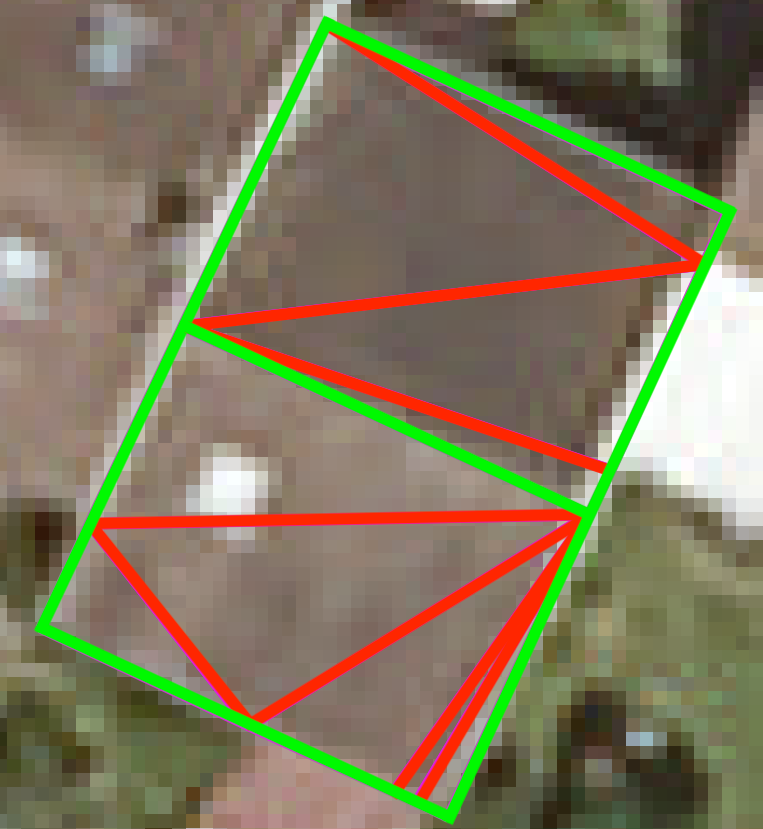
\includegraphics[height=.5\textwidth, width=.5\textwidth]{images/errors/facet/over_segmentation}
                                }{
                                    \caption{
                                        \label{subfig::fos_2d}
                                        A slim chimney in the below corner of the ridge results in a defect ladden \gls{acr::dsm} which translates into an oversegmentation.
                                        The erroneous edges are colored in red.
                                        One can check using the orthoimage that these are not real.
                                    }
                                }
                        \end{subfloatrow}
                    }{
                        \caption{
                            \label{fig::fos}
                            Illustration of a \texttt{\gls{acr::fos}} error.
                        }
                    }
                \end{figure}

                As seen previously, lines are used to help find correct planes and avoid under segmentation.
                However, an overdetection of lines can lead to an oversegmentation of the model.
                This is not rare due to problems that can be encountered with illumination conditions: for instance, a roof structure can cast its shadow on a neighbooring one and cause a gradient in image signal that will be translated to a virtual edge.
                Superstructures play also a negative role just as explained previously.
                This time it is the ones that are small in planar size compared to the noise order of magnitude that are not detected but add bumps that pollute the signal and result in an misestimation of planes.
                High neighbooring buildings are also to blame due to the same reasons as with \texttt{\gls{acr::fus}}, but this time they result in bumps like with superstructures.\\

                To solve this kind of issues, mesh simplification techniques can be helpful.
                In fact,~\textcite{verdie2015lod} uses this approach to smooth away these problems and produce a good generalization of the underlying buildings.
                Another way is to filter the extracted lines relying on redundancy as shown in~\textcite{michelin2013quality}.
                Grammar based methods can equally come to rescue.
                As an example,~\textcite{bredif20073d} uses a set parameteric models in order to model superstructures and better fit \gls{acr::lod}-2 roof facets.

            \paragraph{\texttt{\acrlong*{acr::fib}}.}
                \texttt{\gls{acr::fib}} corresponds to the case where at least one facet border is incorrectly located.
                As an example, Figure~\ref{subfig::fib_2d} shows that the central edge that links the two main roof sides does not correspond to the one on the image position.
                This is a purely geometrical error similarly to \texttt{\gls{acr::bib}}.\\

                \begin{figure}[htbp]
                    \centering
                    \ffigbox[\textwidth]{
                        \begin{subfloatrow}
                            \ffigbox[.5\textwidth]{
                                \includestandalone[mode=buildnew, width=.45\textwidth]{figures/errors/facet/correct_fos_fus_fib_fig}
                            }{
                                \caption{
                                    \label{subfig::gt_fib_3d}
                                    Ground truth \gls{acr::3d} model.
                                }
                            }
                            \ffigbox[.5\textwidth]{
                                \includestandalone[mode=buildnew, width=.45\textwidth]{figures/errors/facet/fib}
                            }{
                                \caption{
                                    \label{subfig::fib_3d}
                                    \gls{acr::3d} model with a \texttt{\gls{acr::fib}} error.
                                    The misplaced edge is colored in red.
                                }
                            }
                        \end{subfloatrow}
                        \vskip1em
                        \begin{subfloatrow}
                                \centering
                                \ffigbox[.75\textwidth]{
                                    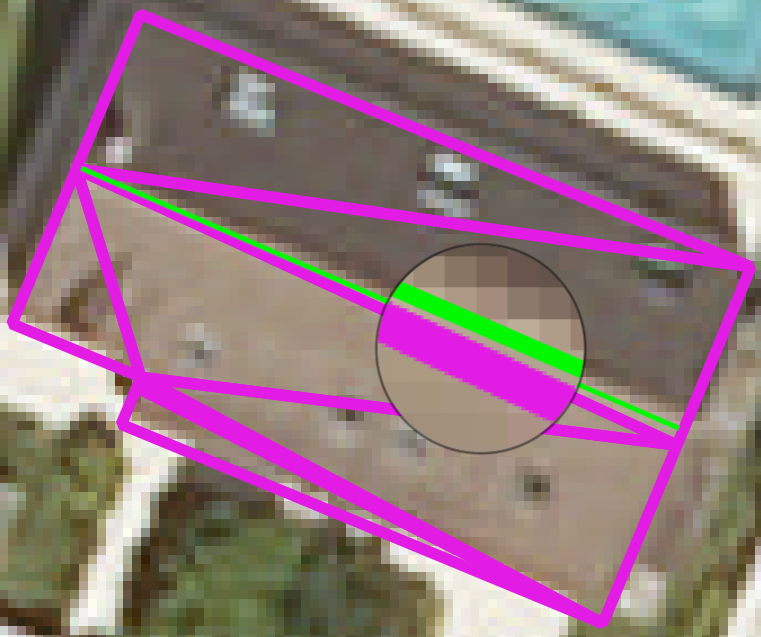
\includegraphics[width=.5\textwidth]{images/errors/facet/border}
                                }{
                                    \caption{
                                        \label{subfig::fib_2d}
                                        The nadir projection of the model on the orthoimage provides the real location (in green) of the edge.
                                    }
                                }
                        \end{subfloatrow}
                    }{
                        \caption{
                            \label{fig::fib}
                            Illustration of a \texttt{\gls{acr::fib}} error.
                        }
                    }
                \end{figure}

                Line extraction is usually very faithfull to the data and depends mostly on the resolution and quality of the input data used for modeling.
                The most likely reason usually behind this kind of errors is usually imprecise fitting of primitives that leads to a shifted intersecting edge such as shown in Figure~\ref{subfig::fib_2d}.\\

                Just as with oversegmentation, one way to make line retrieval more accurate is to rely on redundancy by extracting them from different modalities.
                An alternative is to rely on symmetries~\parencite{verma20063d} to automatically correct surface intersections.

            \paragraph{\texttt{\acrlong*{acr::fit}}.}
                \texttt{\gls{acr::fit}} corresponds to the case where the facet suffers from topological defects such as wrong primitive fitting (for example, a dome approximated by planar polygons).
                In Figure~\ref{fig::fit}, we can observe how two cylindrical towers were reconstructed as a rectangular parallelepiped.\\

                \begin{figure}[htbp]
                    \centering
                    \ffigbox[\textwidth]{
                        \begin{subfloatrow}
                            \ffigbox[.5\textwidth]{
                                \includestandalone[mode=buildnew, width=.45\textwidth]{figures/errors/facet/correct_fit}
                            }{
                                \caption{
                                    \label{subfig::gt_fit_3d}
                                    Ground truth \gls{acr::3d} model.
                                }
                            }
                            \ffigbox[.5\textwidth]{
                                \includestandalone[mode=buildnew, width=.45\textwidth]{figures/errors/facet/fit}
                            }{
                                \caption{
                                    \label{subfig::fit_3d}
                                    \gls{acr::3d} model with a \texttt{\gls{acr::fit}} error.
                                    The facet in yellow has a missing hole.
                                }
                            }
                        \end{subfloatrow}
                        \vskip1em
                        \begin{subfloatrow}
                                \centering
                                \ffigbox[.75\textwidth]{
                                    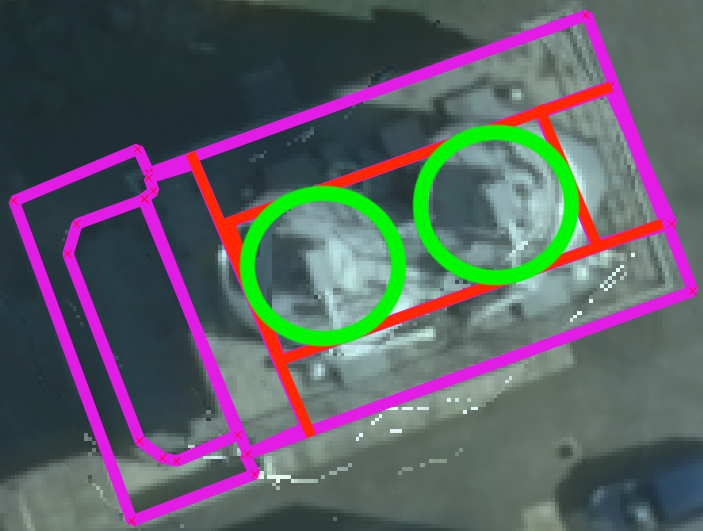
\includegraphics[width=.5\textwidth]{images/errors/facet/topology}
                                }{
                                    \caption{
                                        \label{subfig::fit_2d}
                                        The nadir projection reveals the true form (in green) of the towers that were completly misrepresented (in red).
                                    }
                                }
                        \end{subfloatrow}
                    }{
                        \caption{
                            \label{fig::fit}
                            Illustration of a \texttt{\gls{acr::fit}} error.
                        }
                    }
                \end{figure}

                This can be due to various reasons.
                Most methods rely on the assumption that buildings are piecewise linear~\parencite{nan2017polyfit} or Manhattan-world like~\parencite{li2016manhattan}.
                This is evidently not always the case (cf. Figure~\ref{subfig::fit_2d}).
                Even with the right assumptions, this specific case cannot have been well modeled.
                If so it would have at least approximated the circular cylindrical structures with a regular polygon cylinder.
                This is due to the fact that the quality of the data was poor and was unreliable as explained in the \texttt{\gls{acr::fus}} case in Figure~\ref{subfig::fus_2d}.
                The same effect can cause a missing hole being undetected.\\

                Solving this issue is hard besides the obvious change of primitive assumptions.
                It depends highly on the quality of the data.
                One can try to overcome this issue once again, like with the undersegmentation problem, thanks to line detections to reveal convoluted structures when relying on plane extraction only.
                Usually, this problem can be efficiently solved relying mainly on human operators.

            \paragraph{\texttt{\acrlong*{acr::fig}}.}
                \texttt{\gls{acr::fig}} corresponds to the case of inaccurate facet geometric estimation.
                In mathematical terms, this means that the surface primitive parameters are misestimated.
                In Figure~\ref{subfig::fig_3d}, the planar surface slope was miscalculated as flat while it was of \textit{ca.} \SI{25}{\degree}.\\

                \begin{figure}[htbp]
                    \centering
                    \ffigbox[\textwidth]{
                        \begin{subfloatrow}
                            \ffigbox[.5\textwidth]{
                                \includestandalone[mode=buildnew, width=.45\textwidth]{figures/errors/facet/correct_fos_fus_fib_fig}
                            }{
                                \caption{\label{subfig::gt_fig_3d} Ground truth \gls{acr::3d} model.}
                            }
                            \ffigbox[.5\textwidth]{
                                \includestandalone[mode=buildnew, width=.45\textwidth]{figures/errors/facet/fig}
                            }{
                                \caption{
                                    \label{subfig::fig_3d}
                                    \gls{acr::3d} model with a \texttt{\gls{acr::fig}} error.
                                    The facet in purple has a wrong slope: It is flat instead of being sloped.
                                }
                            }
                        \end{subfloatrow}
                        \vskip1em
                        \begin{subfloatrow}
                                \centering
                                \ffigbox[.75\textwidth]{
                                    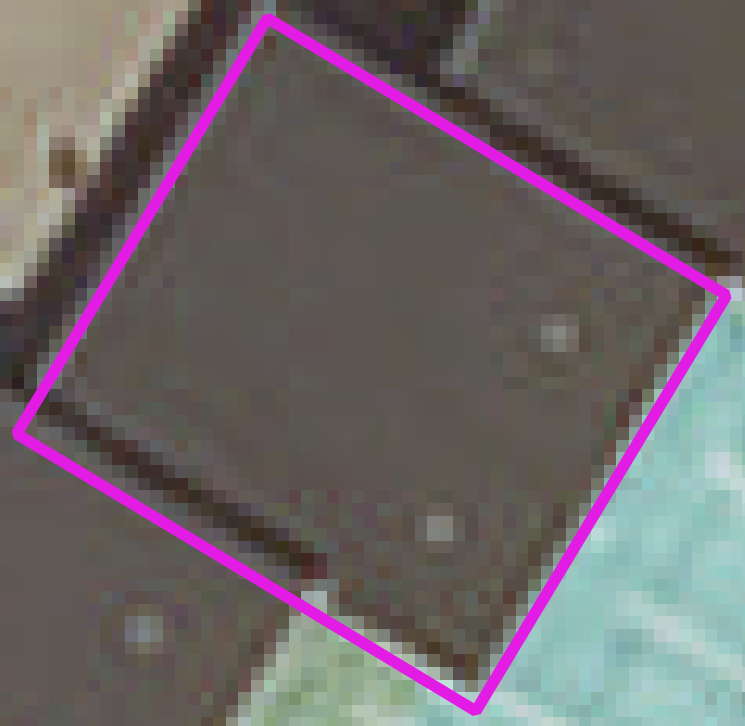
\includegraphics[width=.5\textwidth]{images/errors/facet/geometry}
                            }{
                                \caption{
                                    \label{subfig::fig_2d}
                                    This kind of error is impossible is vizualize on the orthoimage.
                                    Projected on the \gls{acr::dsm}, we can reveal the sloped character of the face.
                                }
                            }
                        \end{subfloatrow}
                    }{
                        \caption{
                            \label{fig::fig}
                            Illustration of a \texttt{\gls{acr::fig}} error.
                        }
                    }
                \end{figure}

                This is linked in particular to the input sensor data quality.
                The case of Figure~\ref{subfig::fig_2d} illustrates how neighbooring building parts influence the data as it blunts away the slope of the roof.
                Semantics play again a role in detecting a purely geometric error.
                For correction, as the corruption in the data resulting from the modeling limits could be filtered out using semantics, one can reestimate the parameters of the primitives.
                Failing that, this correction step is usually conducted by human operators.

    \subsection{Discussion}
        \label{subsec::semantic_evaluation::overhead::discussion}

        In the previous subsection, we defined \texttt{atomic} errors based on our observations related to automatic overhead modeling of urban scenes.
        We also discussed how each type of defects can occur and how to proceed in order to correct them.
        Herein, we explore the properties of the ensuing taxonomy of errors.
        In addition, we also discuss the relation between this taxonomy and the ones existing in the litterature.

        \subsubsection{Error taxonomy properties.}
            The similarity of the \texttt{Building Errors} and \texttt{Facet Errors} is striking.
            Indeed, this is what was intended.
            The idea came after observing that segmentation issues can occur both at building and facet errors.
            It was ruled that both should be separated as they occur at different \glspl{acr::lod} so as to have a fine representation of those defects as discussed in Section~\ref{subsec::semantic_evaluation::general_framework::error_classification}.
            If \texttt{atomic} errors are defined on particular defects observed only at a certain level, one can expect that these definitions are going to be too specific and not exhaustive enough.
            This was the case of an earlier categorization of errors based only on a smaller subset of our datasets~\parencite{ennafii2018semanticunannotated}.
            For instance, at building level, in our dataset, missing courts are fairly present.
            However, there are no cases where facets have holes like illustrated in Figure~\ref{subfig::facet_hole}.
            Both can be grouped in one single label ``missing hole''.
            This example, illustrated in Figure~\ref{fig::holes_levels}, makes the case for using similarity across \glspl{acr::lod} being instrumental for generalizability.\\
            This will also be an interesting option to use even if the error families were different as was proposed in Section~\ref{subsec::semantic_evaluation::general_framework::error_classification}.\\

            \begin{figure}[htbp]
                \centering
                \ffigbox[\FBwidth]{
                    \begin{subfloatrow}[2]
                        \ffigbox[\FBwidth]{
                            \includestandalone[mode=buildnew, width=.45\textwidth]{figures/errors/holes/building}
                        }{
                            \caption{
                                \label{subfig::building_hole}
                                A hole at building (viewed from the top) level (\gls{acr::lod}-1) corresponds to an internal court.
                            }
                        }
                        \ffigbox[\FBwidth]{
                            \includestandalone[mode=buildnew, width=.45\textwidth]{figures/errors/holes/facet}
                        }{
                            \caption{
                                \label{subfig::facet_hole}
                                Example of a facet (\gls{acr::lod}-2) with a rectangular hole corresponding to a balcony.
                            }
                        }
                    \end{subfloatrow}
                }{
                    \caption{
                        \label{fig::holes_levels}
                        Holes observed at different \glspl{acr::lod}.
                    }
                }
            \end{figure}

            Defining errors in \gls{acr::3d} is not an easy task.
            The \textit{implicit} semantics, discussed in Section~\ref{subsubsec::introduction::urban_3d_reconstruction::building_3d_modeling::semantics}, implies the fact that each facet of the model is special and has a meaning.
            Each facet contained in the model is, hence, supposed to be unique and persistent: it cannot be replaced by an approximating set of different facets as in a mesh.
            This meant that evaluating a whole building model amounts to evaluating each facet individually.
            This simplifies greatly the issue as one can think about the problem moslty as a \gls{acr::2d} evaluation one.
            In fact, the first four \texttt{atomic} errors, at each level, involve only \gls{acr::2d} sufaces, which in the case of planar surfaces amount to polygon evaluation.
            The last error is the only one that takes into account the \gls{acr::3d} ascpect of the facets.
            This explains why border imprecisions (which are geometric issues) were separated from the other geometric inaccuracies.
            These latter errors are, in fact, somewhat overlapping.
            These discussed properties does not only help the generalizability and exhaustivity in the overhead case, but can also be applied to terrestrial based fa\c{c}ade modeling.
            In fact, the same \texttt{atomic} errors can describe perfectly the possible errors that can affect facets on a fa\c{c}ade, owing always to the effect of \textit{implicit} semantics on building models.
        
        \subsubsection{Related taxonomies.}
            This Section discusses the semantic error defnitions in the state-of-the-art.
            As mentioned in Section~\ref{subsec::state_of_the_art::quality::output::semantic},~\textcite{rottensteiner2012isprs} proposed two semantic errors ``over segmentation'' and ``under segmentation''.
            These, however, relate only to facets.
            \textcite{xiong2014graph}, although not aiming at evaluating the quality of a model in its entirety, provides some error labels relative to their reconstruction method.
            For instance, ``Missing Node'' (\textit{resp.} ``False Node'', ``Missing Edge'' and ``False Edge'') correspond to, or are included in, the topological \texttt{atomic} errors from the \texttt{Facet Errors} family: \texttt{\gls{acr::fus}} (\textit{resp.} \texttt{\gls{acr::fos}}, \texttt{\gls{acr::fit}}, and \texttt{\gls{acr::fit}}).\\

            On the other hand, the taxonomy developed by~\textcite{michelin2013quality} is the closest to ours.
            In fact, footprint errors could be reshuffled into \texttt{Building Errors} as \texttt{\gls{acr::bib}} (``erroneous outline'' and ``imprecise footprint'') and \texttt{\gls{acr::bit}} (``missing inner court'').
            Intrinsic reconstruction errors are divided into both levels.
            In fact, ``over-segmentation'', ``under segmentation'' could be part of both \texttt{Building Errors} as well as \texttt{Facet Errors} families.
            ``inaccurate roof'' is a general error that can include \texttt{\gls{acr::fib}} and possibly \texttt{\gls{acr::fit}} also.
            ``Z translation'' is the last label in ``Reconstruction errors'' and is either a \texttt{\gls{acr::big}} error when working at \gls{acr::lod}-0 $\cup$ \gls{acr::lod}-1 level, or included into \texttt{\gls{acr::fig}} if dealing with flat roof facets.
            Finally, ``vegetation occlusion'' and `` non existing'' are gathered into the \texttt{Unqualifiable} label at \texttt{finesse} level 0.\\

            Last,~\textcite{boudet2006supervised} studied rather the acceptability of a model as a whole.
            Confidence in a building model is a subjective assessment of building models that depend on the end user needs.
            Consequently, such a taxonomy cannot directly fit with our labels.
            The acceptability dimension can be incorporated into our framework by attributing a confidence score to each error: for example, a prediction probability.        

\section{Parametric label extraction}
    \label{sec::semantic_evaluation::label_extraction}
    When evaluating building models, not all errors are taken into account depending on the end user needs.
    In fact, labels are extracted according to the taxonomy based on the evaluation settings.
    We will see in this subsection how this is possible and what are the consequences of this choice.

    \subsection{Evaluation parameters}
        At evaluation time, three parameters play a role in determining which error labels to consider.
        We determine hereafter these parameters and their role.\\

        The first parameter is the \textbf{\gls{acr::elod}}.
        Every reconstruction method targets a certain set of \glspl{acr::lod}.
        In consequence, when assessing a reconstruction, a \gls{acr::lod} must be specified.
        At a given \gls{acr::elod}, all error families involving higher orders will be ignored.\\
        Depending on the target of the qualification process, a \texttt{finesse} level might be preferred.
        This corresponds to the second parameter called \textbf{\gls{acr::efin}}.
        It specifies the appropriate semantic level at which errors will be reported.\\
        The last one is error \textbf{exclusivity}.
        It derives from the established family error hierarchy.
        If \textbf{exclusivity} is set \textsc{on} errors of a given \gls{acr::lod}-$l$ family are prioritized over ones with higher \glspl{acr::lod}: i.e., \gls{acr::lod} > \gls{acr::lod}-$l$.
        The latter are simply ignored.
        This would useful in the case where the quality evaluation is used by a correction module, either manually or automatically operated.
        In this case, the latter should prioritize solving low \gls{acr::lod} errors rather than trying to solve more detailed ones.
        This stems from the fact that dealing whith low \gls{acr::lod} errors would probably impact the shape of higher \gls{acr::lod} features.
        As a consequence, detecting and correcting the latter rather than prioritizing the low \gls{acr::lod} ones is going to be virtually wasteful in ressources.

    \subsection{Evaluation labels}
        Depending on the previously defined parameters, the considered labels that will be used for the evaluation would differ.
        We will visit herein all the possible cases based on the defined taxonomy for the overhead reconstruction case (cf. Figure~\ref{fig::taxonomy}).
        For this purpose we must first define the function $\operatorname{children}$ that gives the children of a non-leaf node in the taxonomy tree and outputs the same node if it is a leaf:
        \begin{equation}
            \label{eq::children_taxonomy}
            \begin{aligned}
                \operatorname{children}: V &\rightarrow V\\
                n &\mapsto \begin{cases}
                    \left\{n\right\} & n \in L\\
                    \left\{m \in V : (n, m) \in E \right\} & n \notin L
                \end{cases}
            \end{aligned}.
        \end{equation}
        where:
        \begin{conditions}
            V & is the set of all vertices of the taxonomy tree;\\
            L & is the set of leaf nodes in the tree;\\
            E & is the set of edges (directed) in the tree.
        \end{conditions}
        There are eight cases corresponding to one for the case \textbf{\gls{acr::efin}} = 1, three for the error families level and four for the last case of \texttt{atomic} error level.
        
        \begin{enumerate}[label=\roman*)]
            \item \textbf{\gls{acr::efin}} = 1.
                    The model can either be \texttt{Valid} or \texttt{Erroneous}.
                    As discussed previously, most quality evaluation methods reason at this level.
            \item \textbf{\gls{acr::efin}} = 2 and \textbf{\gls{acr::elod}} = \gls{acr::lod}-1.
                    The model can either be \texttt{Valid} or have a \texttt{Building Error}.
            \item \textbf{\gls{acr::efin}} = 2, \textbf{\gls{acr::elod}} = \gls{acr::lod}-2 and the \textbf{exclusivity} is \textsc{on}.
                    The model can either be \texttt{Valid}, have a \texttt{Building Error} or a \texttt{Facet Error}.
            \item \textbf{\gls{acr::efin}} = 2, \textbf{\gls{acr::elod}} = \gls{acr::lod}-2 and the \textbf{exclusivity} is \textsc{off}.
                    The model can either have a \texttt{Building Error} or not.
                    Independently, it can have also a \texttt{Facet Error} or not.
            \item \textbf{\gls{acr::efin}} = 3, \textbf{\gls{acr::elod}} = \gls{acr::lod}-1 and the \textbf{exclusivity} is \textsc{on}.
                    The model can either be \texttt{Valid} or have a \texttt{Building Error}.
                    If the latter is the case, then it is decided if the building model has a \gls{acr::lod}-1 \texttt{atomic} error or not.
                    All the latter errors are considered independently from each other.
            \item \textbf{\gls{acr::efin}} = 3, \textbf{\gls{acr::elod}} = \gls{acr::lod}-1 and the \textbf{exclusivity} is \textsc{off}.
                    The model can have each \gls{acr::lod}-1 \texttt{atomic} error or not independently from the others.
            \item \textbf{\gls{acr::efin}} = 3, \textbf{\gls{acr::elod}} = \gls{acr::lod}-2 and the \textbf{exclusivity} is \textsc{on}.
                    The model can either be \texttt{Valid}, have a \texttt{Building Error} or a \texttt{Facet Error}.
                    If it is affected with a \texttt{Building Error}, then only its corresponding \texttt{atomic} errors are considered being present or not independently.
                    The same decision is applied if \texttt{Facet Error} was detected, but this time with \gls{acr::lod}-2 \texttt{atomic} errors.
            \item \textbf{\gls{acr::efin}} = 3, \textbf{\gls{acr::elod}} = \gls{acr::lod}-2 and the \textbf{exclusivity} is \textsc{off}.
                    The model can have each \texttt{atomic} error (\gls{acr::lod}-1 and \gls{acr::lod}-2) or not independently from the others.
        \end{enumerate}

        This will influence the evaluation pipeline that will be described later in the next chapter.
        Indeed, the latter will provide more insight about how this takes place.
